\documentclass[compress]{beamer}
\usepackage{ifthen,verbatim}

\title{Muon Alignment Progress}
\author{Jim Pivarski, Alexei Safonov}
\institute{Texas A\&M University}
\date{24 January, 2008}

\newcommand{\isnote}{}
\xdefinecolor{lightyellow}{rgb}{1.,1.,0.25}
\xdefinecolor{darkblue}{rgb}{0.1,0.1,0.7}

%% Uncomment this to get annotations
%% \def\notes{\addtocounter{page}{-1}
%%            \renewcommand{\isnote}{*}
%% 	   \beamertemplateshadingbackground{lightyellow}{white}
%%            \begin{frame}
%%            \frametitle{Notes for the previous page (page \insertpagenumber)}
%%            \itemize}
%% \def\endnotes{\enditemize
%% 	      \end{frame}
%%               \beamertemplateshadingbackground{white}{white}
%%               \renewcommand{\isnote}{}}

%% Uncomment this to not get annotations
\def\notes{\comment}
\def\endnotes{\endcomment}

\setbeamertemplate{navigation symbols}{}
\setbeamertemplate{headline}{\includegraphics[height=1 cm]{../cmslogo} \hspace{0.1 cm} \includegraphics[height=1 cm]{../tamulogo} \hfill
\begin{minipage}{5.5 cm}
\vspace{-0.75 cm} \small
\begin{center}
\ifthenelse{\equal{\insertpagenumber}{1}}{}{\textcolor{blue}{\insertsection}}
\end{center}
\end{minipage} \hfill
\begin{minipage}{4.5 cm}
\vspace{-0.75 cm} \small
\begin{flushright}
\ifthenelse{\equal{\insertpagenumber}{1}}{}{Jim Pivarski \hspace{0.5 cm} \insertpagenumber\isnote/\pageref{numpages}}
\end{flushright}
\end{minipage}\mbox{\hspace{0.2 cm}}}

\begin{document}
\frame{\titlepage}

%% \begin{notes}
%% \item This is the annotated version of my talk.
%% \item If you want the version that I am presenting, download the one
%% labeled ``slides'' on Indico (or just ignore these yellow pages).
%% \item The annotated version is provided for extra detail and a written
%% record of comments that I intend to make orally.
%% \item Yellow notes refer to the content on the {\it previous} page.
%% \item All other slides are identical for the two versions.
%% \end{notes}

\begin{frame}
\frametitle{In a nutshell}
\begin{itemize}\setlength{\itemsep}{0.35 cm}
\item The last time I presented was in November

\vspace{0.1 cm}
I had optimized existing code for 10~pb$^{-1}$ alignment

\item Since then, I have scaled up to 100~pb$^{-1}$ and see only
marginal improvement in alignment quality (not $\sqrt{10}$)

\item Re-tuning parameters for 100~pb$^{-1}$ helps

\item So do new tools: track filter and alignment-specific refitter,
but these are still experimental

\item Currently parallelizing the baseline procedure so that I can
study improvements in a controlled and timely fashion
\end{itemize}
\end{frame}

\begin{frame}
\frametitle{Reminder of the method}
\begin{itemize}\setlength{\itemsep}{0.35 cm}
\item First pass: align whole wheels and disks with loose muon hit
weights in track refits (Alignment Parameter Error or APE~=~2~cm)

\item Second pass: align chambers in inner stations with large APEs

\item Third pass: set inner station APEs~=~0, align chambers in next station

\item Et cetera\ldots

\item Eighth pass: re-align all chambers with small APEs

\item Ninth pass: re-align chambers in all but first stations with small APEs
\end{itemize}
\end{frame}

\section*{Scaling up to 100~pb$^{-1}$}

\begin{frame}
\frametitle{Scaling up to 100~pb$^{-1}$}
\begin{itemize}\setlength{\itemsep}{0.6 cm}
\item CPU-intensive: 9 alignment passes $\times$ 5 iterations each = 45~iterations

\item Developed ``the easy way'' as a single CPU process

\item 100~pb$^{-1}$ took 8 days to process

\vspace{0.1 cm}
(fortunately, this could run over the winter break)

\item Parallelizing to 50 CPUs (= 4 hours) is possible,

\vspace{0.1 cm}
but takes some work to get right (see end of this talk)
\end{itemize}
\end{frame}

\begin{frame}
\frametitle{Side-by-side comparison (alignment position error)}

``Chamber $x$ position RMS'' is $\sqrt{\overline{(x_{\mbox{\scriptsize true}} - x_{\mbox{\scriptsize aligned}})^2}}$, includes offsets

\vspace{0.1 cm}
(these are with no tracker misalignment, but the story is the same)

\vspace{-0.2 cm}
\begin{columns}
\column{0.5\linewidth}
\begin{center} \textcolor{darkblue}{10~pb$^{-1}$ alignment} \end{center}

\vspace{-0.25 cm}
\includegraphics[height=\linewidth, angle=90]{convergence-10.pdf}

\column{0.5\linewidth}
\begin{center} \textcolor{darkblue}{100~pb$^{-1}$ alignment} \end{center}

\vspace{-0.25 cm}
\includegraphics[height=\linewidth, angle=90]{convergence-100.pdf}
\end{columns}
\end{frame}

\begin{frame}
\frametitle{Overlaid comparison (alignment position error)}

\begin{center} \textcolor{red}{red: 10~pb$^{-1}$} \hspace{0.5 cm} \textcolor{blue}{blue: 100~pb$^{-1}$}

\includegraphics[height=0.8\linewidth, angle=90]{convergence_overlay.pdf}

\end{center}

\vspace{-0.5 cm}
\begin{itemize}
\item Wheel/disk alignment hasn't converged!  5 $\to$ 15 iterations
\end{itemize}
\end{frame}

\section*{Diagnosis and improvements}

\begin{frame}
\frametitle{Why doesn't it scale with statistics? (\only<1>{1}\only<2>{2})}
\only<1>{\begin{itemize}
\item Clearly {\it some} source of systematic error is drowning out dependence on statistics

\item Strong dependence on APE!

Below, APE = $\infty$ after wheel/disk (dashed line)
\end{itemize}}
\only<2>{\begin{itemize}
\item APE = $\infty$ case improves 100~pb$^{-1}$ alignment and worsens
10~pb$^{-1}$ alignment: scaling is $\sqrt{5}$

\item (APEs had been optimized for 10~pb$^{-1}$\ldots)

\mbox{ }
\end{itemize}}

\vspace{-0.35 cm}
\begin{columns}
\column{0.5\linewidth}
\begin{center} \textcolor{darkblue}{10~pb$^{-1}$ alignment} \end{center}

\vspace{-0.25 cm}
\includegraphics[height=\linewidth, angle=90]{large_APEs-10.pdf}

\column{0.5\linewidth}
\begin{center} \textcolor{darkblue}{100~pb$^{-1}$ alignment} \end{center}

\vspace{-0.25 cm}
\includegraphics[height=\linewidth, angle=90]{large_APEs-100.pdf}
\end{columns}
\end{frame}

\begin{frame}
\frametitle{Something else that helps: cut on tracks}
\begin{columns}
\column{0.4\linewidth}
\includegraphics[width=1.1\linewidth]{trackcut.pdf}

\column{0.65\linewidth}
\begin{itemize}
\item Keep tracks whose last-station residual is within a $\pm 3
\sigma$ window when propagated with APE = $\infty$

\item Tests consistency of real muon (hit) with ideal propagation (no scattering)
\end{itemize}

\vspace{-0.5 cm}
\begin{center} \includegraphics[height=0.77\linewidth, angle=90]{large_APEs_trackcut-100.pdf} \end{center}

\end{columns}
\end{frame}

\begin{frame}
\frametitle{Considerations for the track-cut}
\begin{itemize}\setlength{\itemsep}{0.5 cm}
\item Windows are defined by APE~=~$\infty$ propagations, cut must
only be applied to APE~=~$\infty$ propagations

\item In most passes, tracks must be propagated twice:
\begin{enumerate}
\item once to determine applicability of the cut
\item again in track-fit with APE~=~0 on already-aligned chambers
\end{enumerate}

\item Windows must be redefined every time last stations are moved

\item Mean and stdev are written to a readable-text configuration file for safety
\end{itemize}
\end{frame}

\begin{frame}
\frametitle{Diagnosis via improvements}
\begin{itemize}\setlength{\itemsep}{0.35 cm}
\item Finite APEs reduce statistical errors, but exacerbate systematic effect

%% \begin{columns}
%% \column{0.5\linewidth}
%% Simple $\sqrt{\mbox{stat}^2 + \mbox{syst}^2}$ model:
%% \begin{itemize}
%% \item ``stat'' scales as $\sqrt{10}$

%% \item ``syst'' indep.\ of int.\ lumi
%% \end{itemize}
%% (outermost station presented)

%% \column{0.6\linewidth}
%% 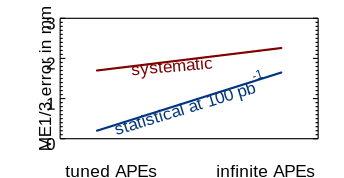
\includegraphics[width=\linewidth]{statsyst.png}
%% \end{columns}

\item Ratio of improvements from track cut in APE~=~$\infty$ test

\vspace{0.2 cm}
\begin{columns}
\column{0.7\linewidth}
\begin{tabular}{c c c c c c}
\hline \hline MB1 & 1.5 & MB2 & 2.7 & MB3 & 1.1 \\\hline
ME1/1 & 1.1 & ME1/2 & 2.4 & & \\
ME2/1 & 1.2 & ME2/2 & 2.2 & & \\
ME3/1 & 1.0 \\\hline \hline
\end{tabular}

\column{0.25\linewidth}
(1.0 is no improvement)
\end{columns}

\item The effect is probably related to scattering

\item But it's not symmetric

\item Amplified in outer stations due to our local-propagation method

\end{itemize}
\end{frame}

\section*{More improvements}

\begin{frame}
\frametitle{Potentially useful: new track refitter}
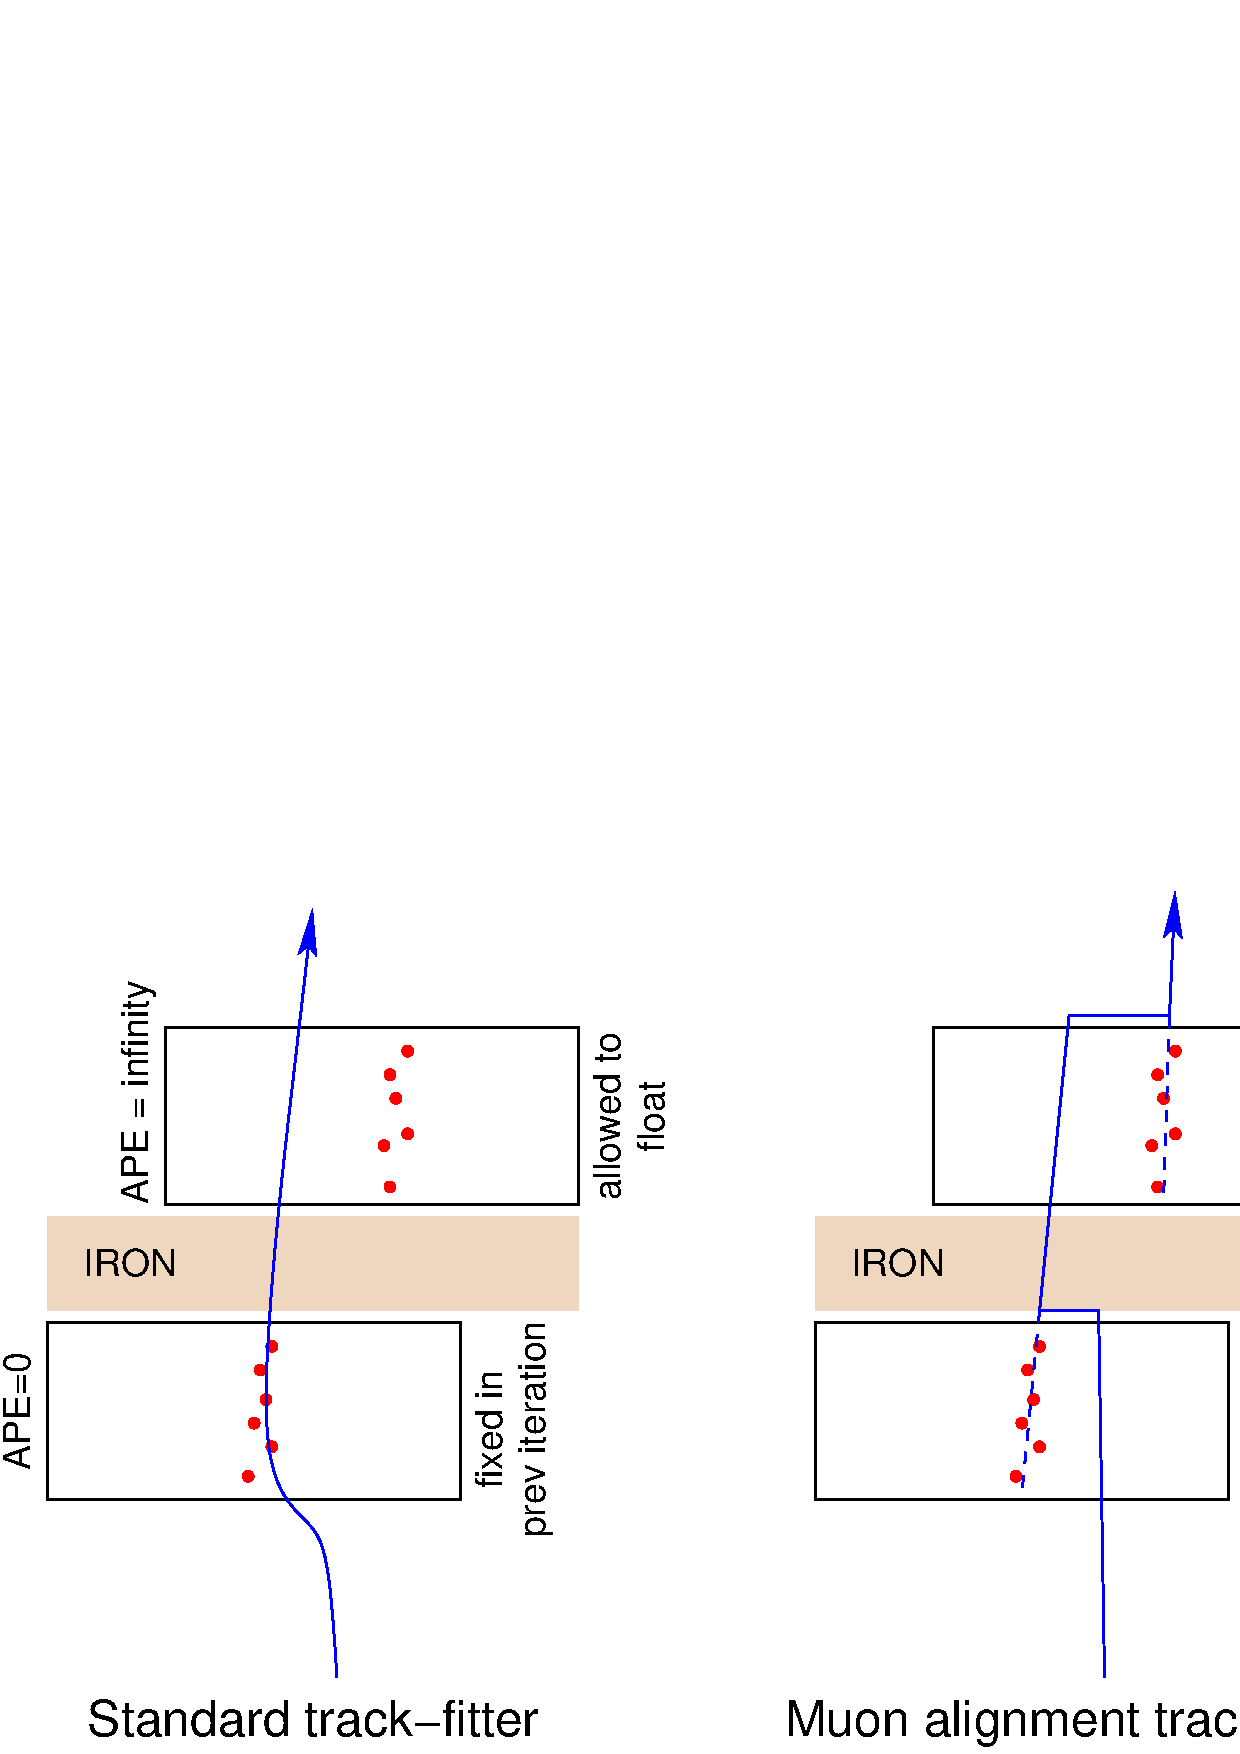
\includegraphics[width=\linewidth]{newtrackfitter.pdf}
\end{frame}

\begin{frame}
\frametitle{New track refitter}
\mbox{ }

\vspace{-1.5 cm}
\mbox{ } \hfill 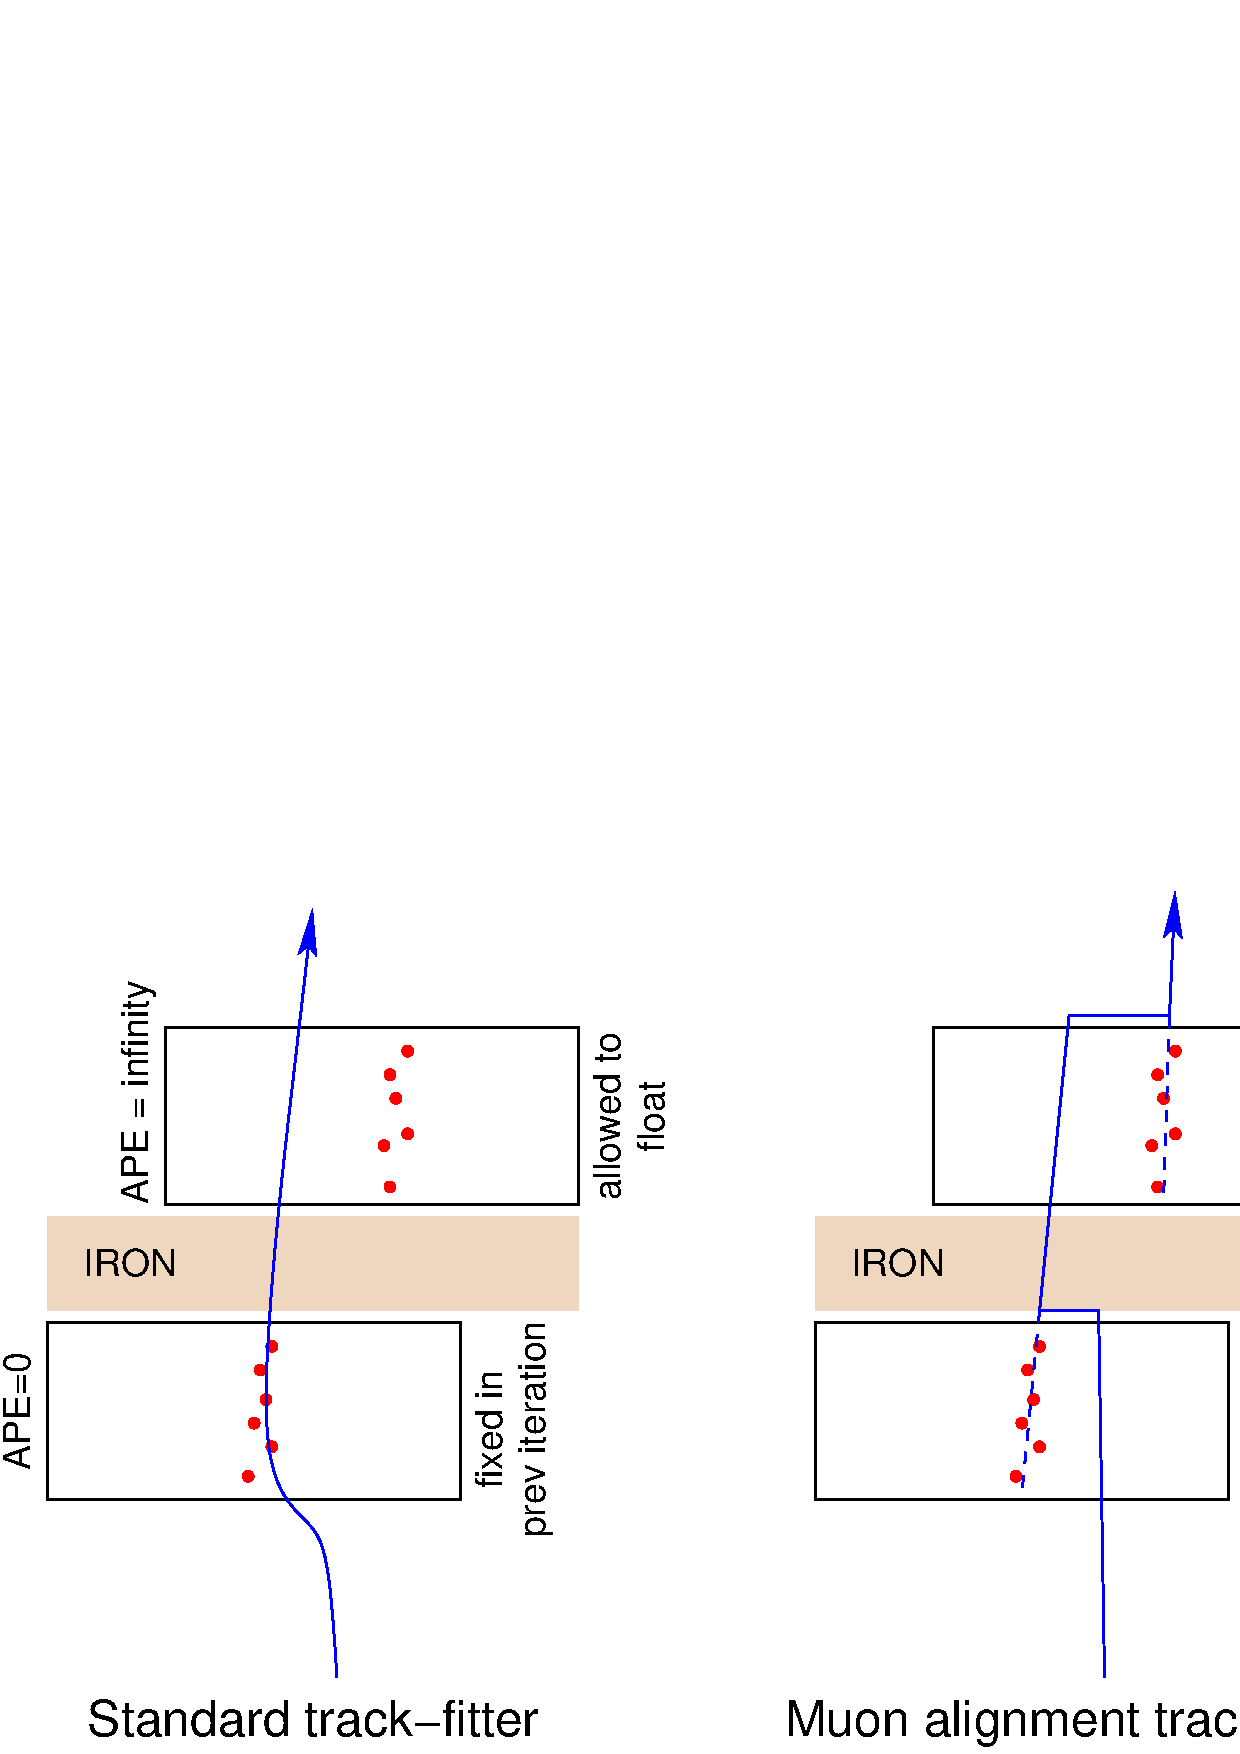
\includegraphics[width=0.5\linewidth]{newtrackfitter.pdf}

\vspace{-2 cm}
\begin{itemize}\setlength{\itemsep}{0.2 cm}
\item Accomplish same \\ local propagation \\ method in one pass \\ (with more iterations)

\item More control over how track is updated:

\vspace{0.1 cm}
Ideally, tracker should fix $|\vec{p}|$, muon chamber should
only update position $(x,y)$ and direction $(\eta,\phi)$

\item This is a generalization of Gena's suggestion to align with overlap hits

\item Implemented, working, but not in ``baseline'' procedure

\item Might only be a convergence-speed improvement; might outperform
baseline method when $\rho(x)$, $\vec{B}(x)$ is uncertain
\end{itemize}
\end{frame}

\section*{Parallelization of baseline procedure}

\begin{frame}
\frametitle{Software: setting up procedure to run in parallel}
\begin{itemize}\setlength{\itemsep}{0.4 cm}
\item Iteration 1 splits into 50 jobs, collected and merged, then on to iteration 2\ldots

\item 2805 configuration files, all different

\item Seems to be working, but CAF stopped accepting my jobs yesterday

\item This is the revised CSA exercise (reporting computing
requirements tomorrow at Al/Ca)

\item With a faster alignment procedure, we can do proper studies of
the systematic error and the improvements discussed in~this~talk
\end{itemize}
\end{frame}

\section*{}

\begin{frame}
\frametitle{Conclusions}
\begin{itemize}\setlength{\itemsep}{0.5 cm}
\item Alignment error is dominated by a {\it reducible} component

\item Origin is unknown, but probably related to scattering tracks

\item New track-level cut helps: added to baseline procedure (width of
window is still unoptimized)

\item New track fitter (already written) may also help, especially if
infinite-APE track-fitting is suspect \\ (e.g.\ uncertain material
$\rho(x)$ or $\vec{B}(x)$ field)

\item {\it Baseline} procedure is conventional: what we have been working
with for 3 months, with loosened APEs and a track cut that can be wide
\end{itemize}
\label{numpages}
\end{frame}

\end{document}
